\chapter{实验与测试}
\label{cha:evaluations}

对上面三章所提的内容,本章将开展四个实验进行综合测试和分析。
首先是GPU渲染器与CPU渲染器之间的性能比较测试,该实验将在同一场景下分别运行本人实现的GPU渲染器和两款主流的CPU渲染器(Mitsuba,Pbrt),
通过比较渲染时间及效果探讨该GPU渲染器的效率优劣;
其次,将利用GPU渲染器对两种已经实现的渲染算法进行对照实验,验证设计算法的正确性;
最后,将围绕第五章中介绍的VRay模拟材质的进行效果测试,并尝试总结其达到的模拟程度以及与VRay原材质之间的主要差异。

以下实验均是在RTX 2080显卡+i9 9900KCPU(16核,3.40GHz)的硬件环境下完成的。

\section{GPU渲染与CPU渲染的性能比较实验}

为了体现测试的公平性,首先需要做出适当的规定,以保证双方渲染算法的一致性。在该实验中,
双方需要运行不包含任何优化的路径追踪算法,以输出分辨率为1280x720的图像;
渲染中所使用的基本参数如材质参数、相机参数、光线最大深度等都应当完全一致。
在以上的这些限制下,两款渲染器需要各自运行256次采样流程,并记录总共花费的时间以进行对比。

然而另一方面,由于不同渲染器的场景输入格式不一,且各渲染器的内部实现也有较大差异,
因此各方的渲染结果很难做到完全一致。在实际操作中,
本人最终选择了三个复杂度各异的场景用来测试:Bedroom、Staircase以及Cornell。
在材质上,本人的GPU渲染器和PBRT渲染器都采用了有严格定义的Disney BRDF材质,
而Mitsuba渲染器由于没有该材质的实现,则使用了更加简单的Lambert材质作为替代。
各个渲染器的运行时间和结果图如表\ref{tab:lab1time}和图\ref{fig:lab1image}所示。

% Please add the following required packages to your document preamble:
% \usepackage{booktabs}
\begin{table}[]
    \centering
    \begin{tabular}{@{}lccc@{}}
    \toprule
    渲染器     &  PBRT & Mitsuba & GPU渲染器 \\ \midrule
    Cornell &   259.9s   &   39.6s   &    \textbf{26.9s}     \\
    Staircase    &   502.6s  &   99.64s  &    \textbf{65.0s}    \\
    Bedroom &   379.2s    &   91.9s    &    \textbf{44.7s}   \\ \bottomrule
    \end{tabular}
    \vspace{2mm}
    \caption{各个渲染器在不同场景下运行同样采样次数的所需时间}
    \label{tab:lab1time}
\end{table}

\begin{figure}                 %%%%%%%% 观测干扰的结果
    \begin{minipage}{0.3\textwidth}  %% {0.18\textwidth}
      \centerline{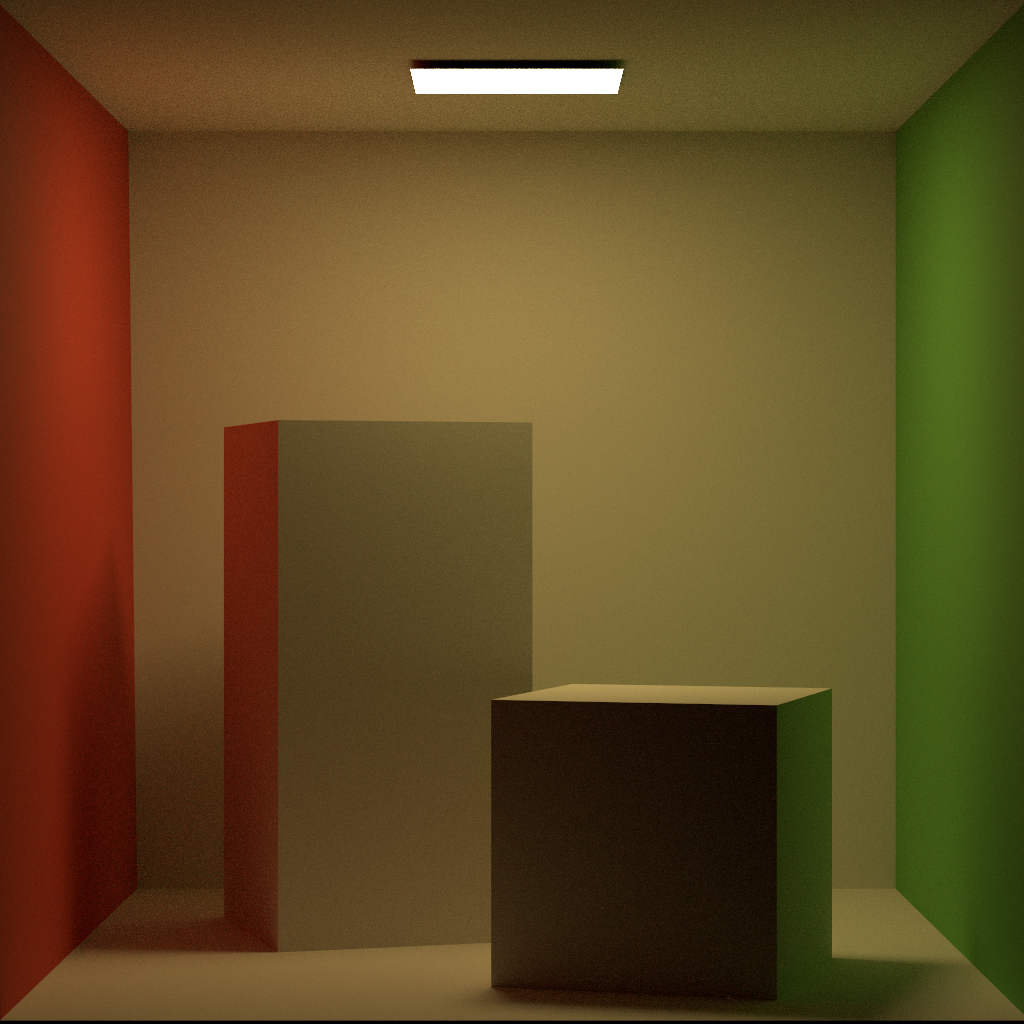
\includegraphics[width=1\textwidth]{evaluationResult/GPU_CPU/cornell-box.jpg}}
      \centerline{(a1)}
    \end{minipage}
    \hfill
    \begin{minipage}{0.3\textwidth}  %% {0.18\textwidth}
      \centerline{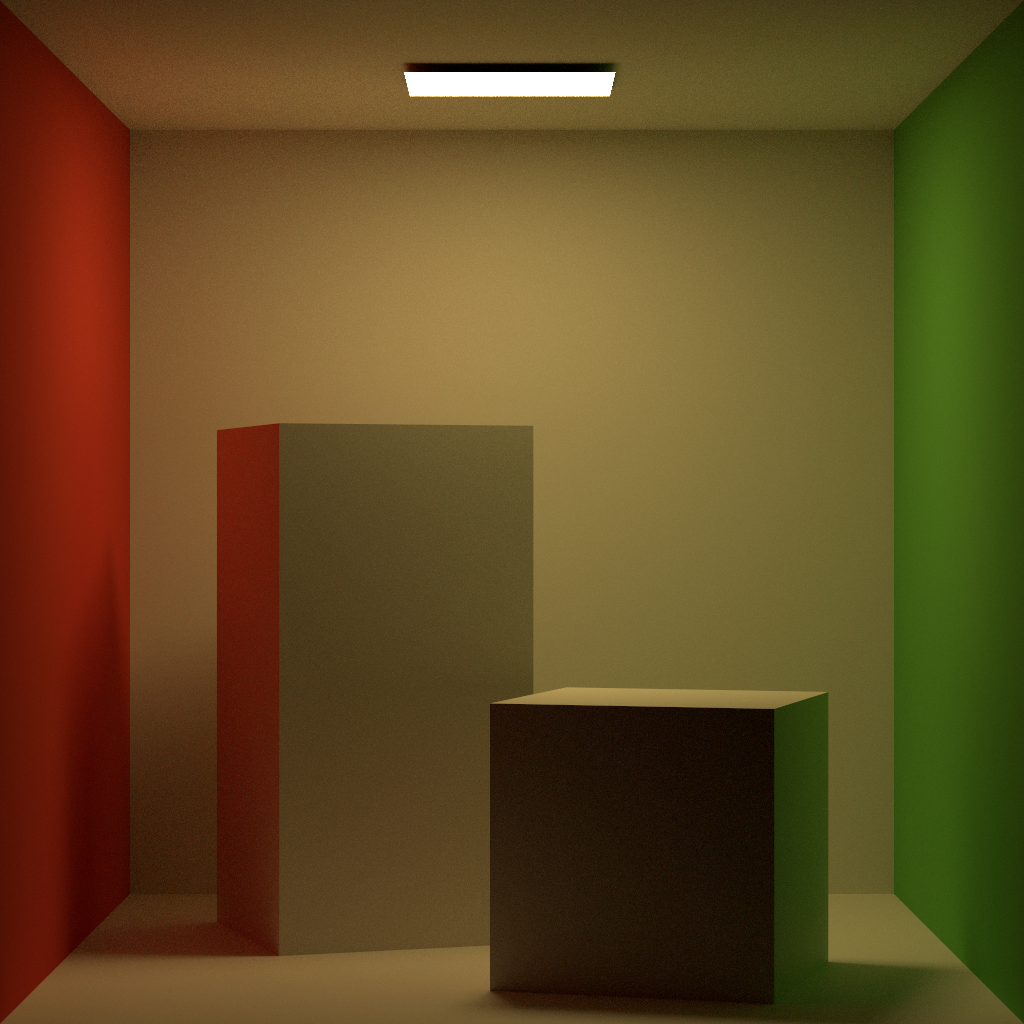
\includegraphics[width=1\textwidth]{evaluationResult/GPU_CPU/cornell-box_pbrt.png}}
      \centerline{(b1)}
    \end{minipage}    
    \hfill
    \begin{minipage}{0.3\textwidth}  %% {0.18\textwidth}
        \centerline{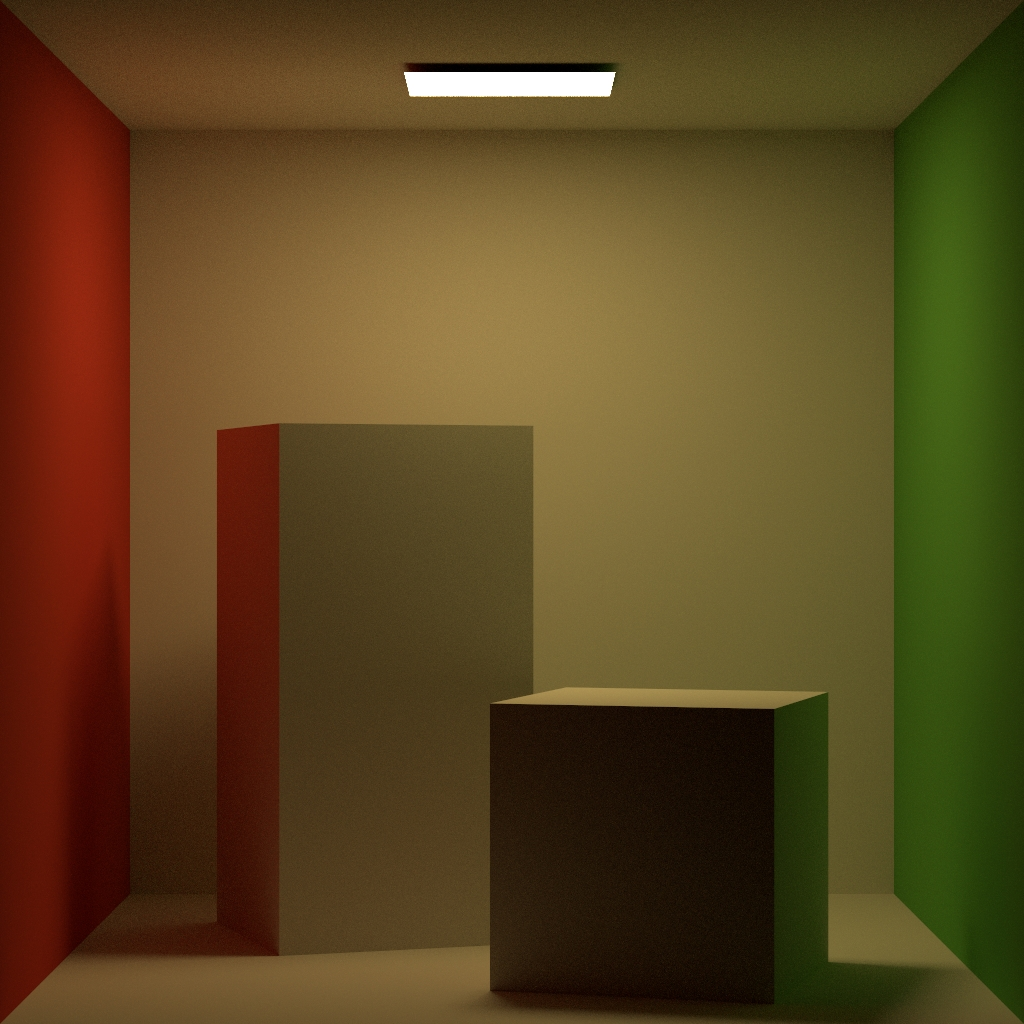
\includegraphics[width=1\textwidth]{evaluationResult/GPU_CPU/cornell-box_mitsuba.jpg}}
        \centerline{(c1)}
      \end{minipage}
    \vfill
    \begin{minipage}{0.3\textwidth}  %% {0.18\textwidth}
        \centerline{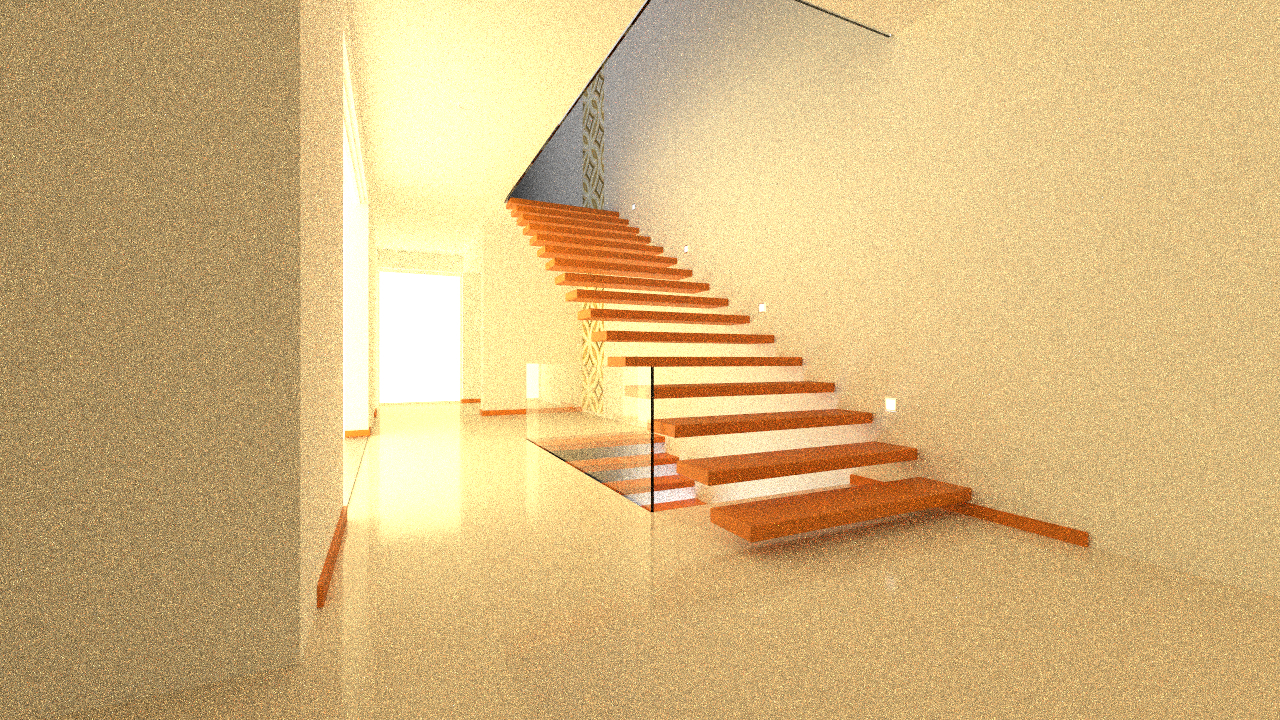
\includegraphics[width=1\textwidth]{evaluationResult/GPU_CPU/1_stair.jpg}}
        \centerline{(a2)}
      \end{minipage}
      \hfill
      \begin{minipage}{0.3\textwidth}  %% {0.18\textwidth}
        \centerline{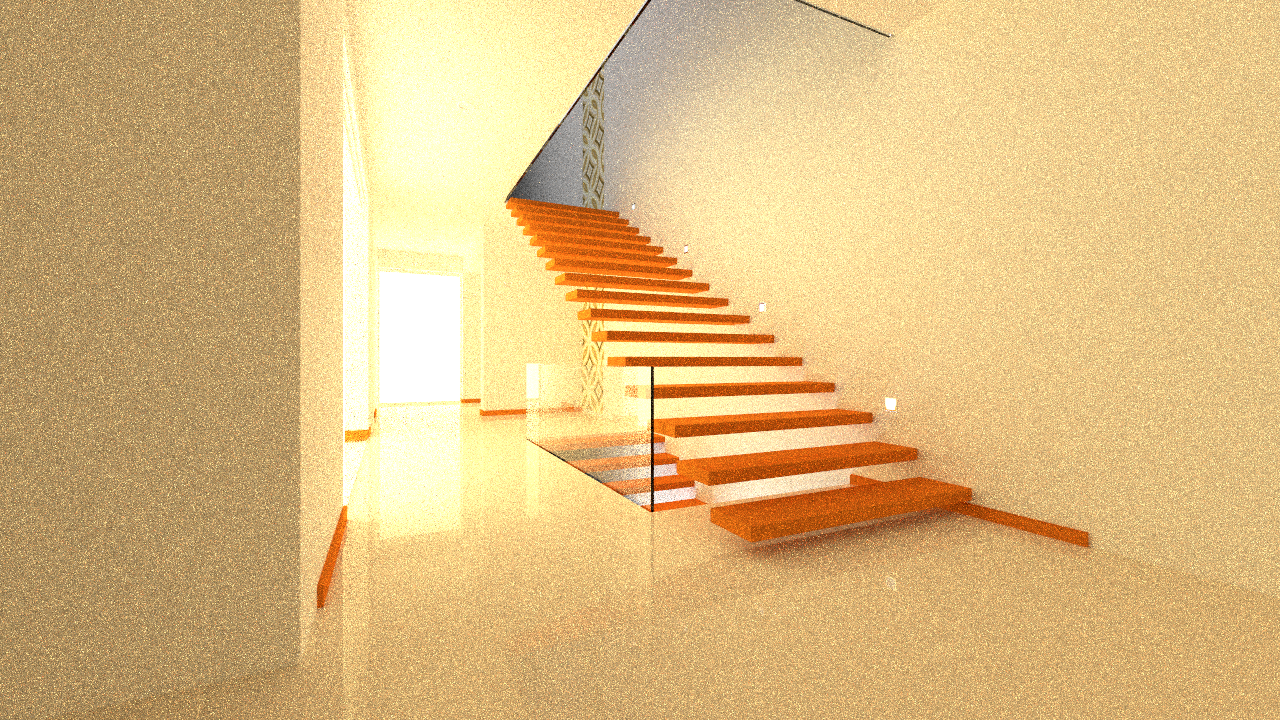
\includegraphics[width=1\textwidth]{evaluationResult/GPU_CPU/1_stair_pbrt.png}}
        \centerline{(b2)}
      \end{minipage}    
      \hfill
      \begin{minipage}{0.3\textwidth}  %% {0.18\textwidth}
          \centerline{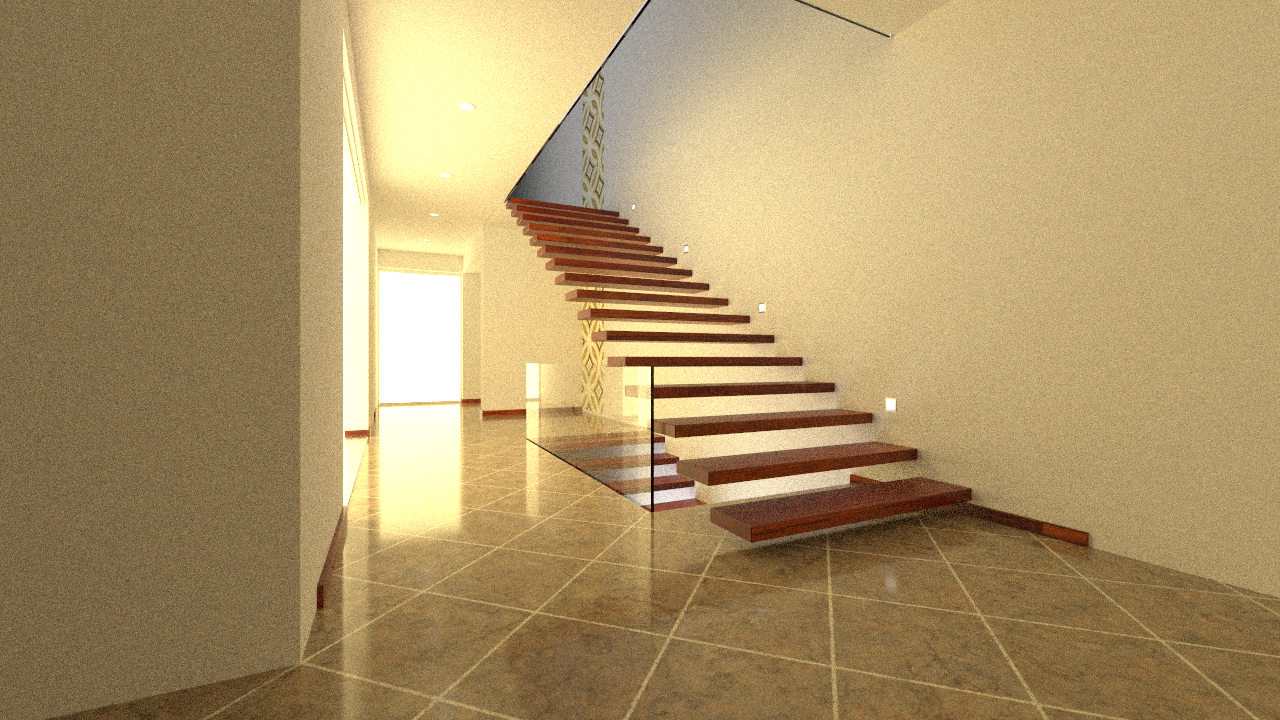
\includegraphics[width=1\textwidth]{evaluationResult/GPU_CPU/1_stair_mitsuba.png}}
          \centerline{(c2)}
        \end{minipage}
      \vfill
    \begin{minipage}{0.3\textwidth}  %% {0.18\textwidth}
    \centerline{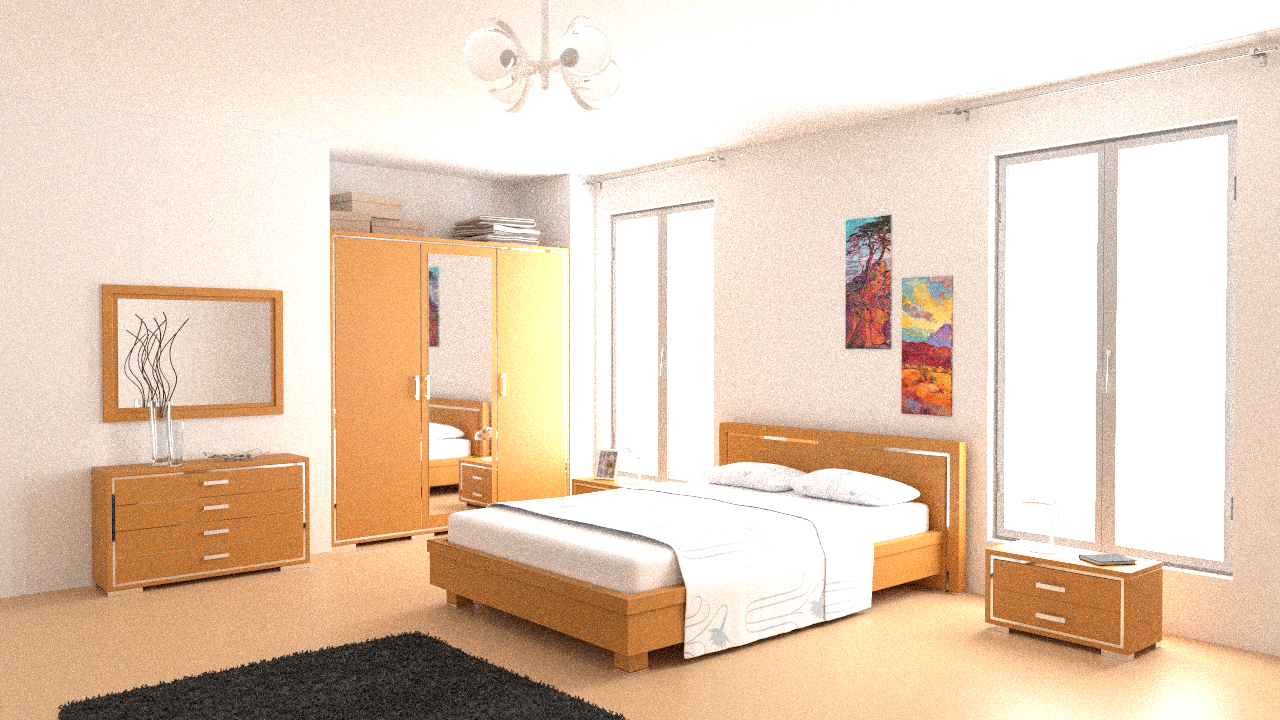
\includegraphics[width=1\textwidth]{evaluationResult/GPU_CPU/1_bedroom.jpg}}
    \centerline{(a3)}
    \end{minipage}
    \hfill
    \begin{minipage}{0.3\textwidth}  %% {0.18\textwidth}
    \centerline{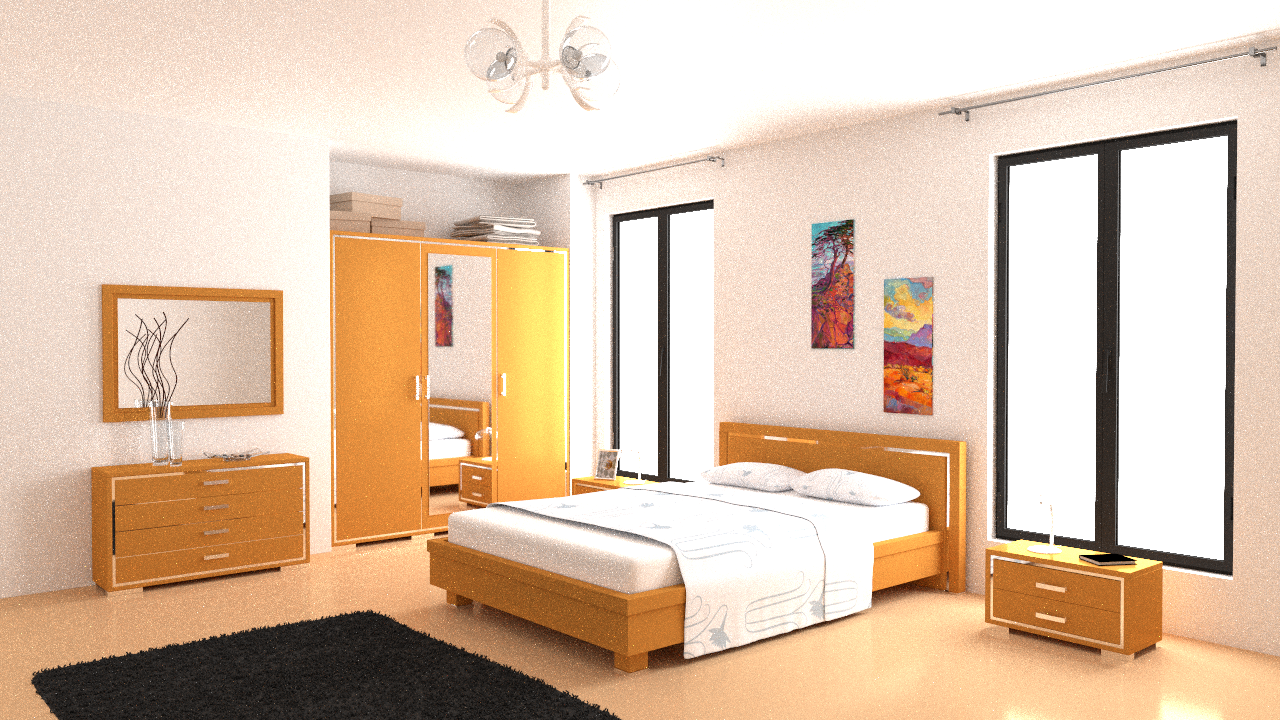
\includegraphics[width=1\textwidth]{evaluationResult/GPU_CPU/1_bedroom_pbrt.png}}
    \centerline{(b3)}
    \end{minipage}    
    \hfill
    \begin{minipage}{0.3\textwidth}  %% {0.18\textwidth}
        \centerline{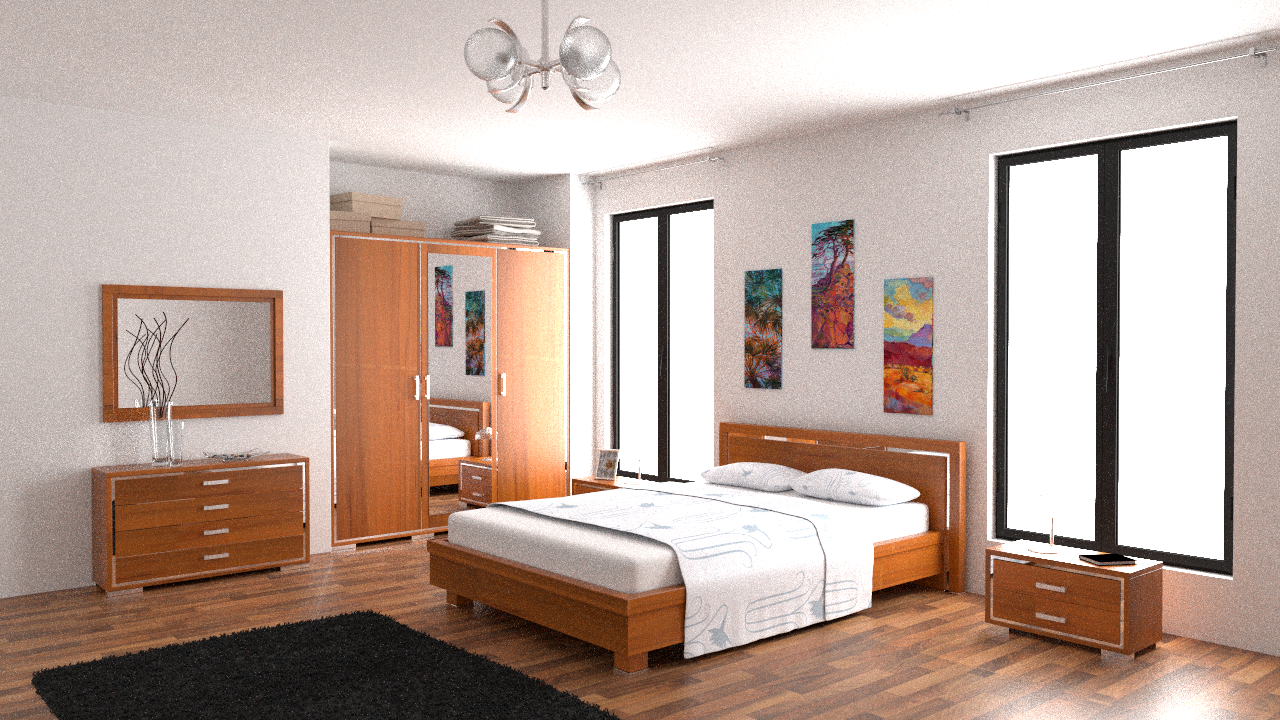
\includegraphics[width=1\textwidth]{evaluationResult/GPU_CPU/1_bedroom_mitsuba.png}}
        \centerline{(c3)}
    \end{minipage}
    \vfill
    \caption{各渲染器的渲染结果。其中,(a1),(a2),(a3)分别代表GPU渲染器在Cornell、Staircase和Bedroom场景下的渲染结果,
    而(b1),(b2),(b3)为PBRT渲染结果,(c1),(c2),(c3)为Mitsuba渲染结果。}
    \label{fig:lab1image}
\end{figure}

从结果图中可以看到,GPU渲染器和PBRT的渲染结果基本一致,而Mistuba渲染器由于材质不同则稍有差异。
另一方面,根据表格的结果,GPU渲染器在速度上唱过了Pbrt数倍,而对于Mitsuba渲染器而言,即使使用了更复杂的材质,GPU渲染器依然获得了更快的速度。
以上的实验结果足以说明,GPU对于光线追踪渲染的效率提升能够起到显著的作用。

\section{路径追踪算法与SPPM算法比较}

路径追踪算法与SPPM算法的目的都是求解渲染方程,因此这两者最后的理论收敛值应当是完全一致的。
因此,本实验将对运行足够长时间的SPPM渲染结果和路径追踪渲染结果进行比较,从而验证双方的实现结果是否符合预期。
另外,还会对SPPM中不同的初始半径对算法结果的影响进行简单的评估。

对于实验的第一部分,本人分别用两个渲染算法渲染了Cornell、Sponza和Bedroom三个场景,
两者的光线最大深度都保持一致(实验中分别被设置为5次)。
同时,为了确保结果收敛,实验中路径追踪算法的迭代次数被设为3000轮,
而SPPM算法由于收敛速度更快,迭代次数则设置为1000轮。
根据场景大小的不同,SPPM算法的初始半径在三个场景中分别被设置为了1000,10000和0.05。
图\ref{fig:lab2image}显示了两个算法的运行结果及差异,
而\ref{tab:lab2time}则是两者的具体运算时间和结果上的差值。

\begin{table}[]
    \centering
    \begin{tabular}{@{}lccc@{}}
    \toprule
    场景     &  Cornell & Sponza & Bedroom \\ \midrule
    路径追踪运行时间 &   281.70s   &   443.13s   &  374.53s  \\
    SPPM运行时间 &   36.7s   &   39.6s  &  37.1s  \\
    相对平方误差(RSE) &   0.001   &   0.013   &  0.015  \\
    \bottomrule
    \end{tabular}
    \vspace{2mm}
    \caption{路径追踪算法和SPPM算法的运算时间及误差情况。}
    \label{tab:lab2time}
\end{table}

\begin{figure}                 %%%%%%%% 观测干扰的结果
    \begin{minipage}{0.3\textwidth}  %% {0.18\textwidth}
      \centerline{\includegraphics[width=1\textwidth]{evaluationResult/SPPM_PT/cornell/pt.jpg}}
      \centerline{(a1)}
    \end{minipage}
    \hfill
    \begin{minipage}{0.3\textwidth}  %% {0.18\textwidth}
      \centerline{\includegraphics[width=1\textwidth]{evaluationResult/SPPM_PT/cornell/sppm.jpg}}
      \centerline{(b1)}
    \end{minipage}    
    \hfill
    \begin{minipage}{0.3\textwidth}  %% {0.18\textwidth}
        \centerline{\includegraphics[width=1\textwidth]{evaluationResult/SPPM_PT/cornell/rse.jpg}}
        \centerline{(c1)}
      \end{minipage}
    \vfill
    \begin{minipage}{0.3\textwidth}  %% {0.18\textwidth}
        \centerline{\includegraphics[width=1\textwidth]{evaluationResult/SPPM_PT/sponza/pt.jpg}}
        \centerline{(a1)}
      \end{minipage}
      \hfill
      \begin{minipage}{0.3\textwidth}  %% {0.18\textwidth}
        \centerline{\includegraphics[width=1\textwidth]{evaluationResult/SPPM_PT/sponza/sppm.jpg}}
        \centerline{(b1)}
      \end{minipage}    
      \hfill
      \begin{minipage}{0.3\textwidth}  %% {0.18\textwidth}
          \centerline{\includegraphics[width=1\textwidth]{evaluationResult/SPPM_PT/sponza/rse.jpg}}
          \centerline{(c1)}
        \end{minipage}
      \vfill
      \begin{minipage}{0.3\textwidth}  %% {0.18\textwidth}
        \centerline{\includegraphics[width=1\textwidth]{evaluationResult/SPPM_PT/bedroom/pt.jpg}}
        \centerline{(a1)}
      \end{minipage}
      \hfill
      \begin{minipage}{0.3\textwidth}  %% {0.18\textwidth}
        \centerline{\includegraphics[width=1\textwidth]{evaluationResult/SPPM_PT/bedroom/sppm.jpg}}
        \centerline{(b1)}
      \end{minipage}    
      \hfill
      \begin{minipage}{0.3\textwidth}  %% {0.18\textwidth}
          \centerline{\includegraphics[width=1\textwidth]{evaluationResult/SPPM_PT/bedroom/rse.jpg}}
          \centerline{(c1)}
        \end{minipage}
      \vfill
    \caption{两种渲染算法的结果及差异情况。上图中,左侧图像(a1-a3)为SPPM算法生成,中测图像(b1-b3)为路径追踪算法生成,
    而右侧图像(c1-c3)则为两张图像的相对平方误差值(Related Square Error)。}
    \label{fig:lab2image}
\end{figure}

从结果图中可以看出,SPPM算法图像中的噪声相比路径追踪算法要柔和许多,但在一些特殊区域如角落却显得十分阴暗。
这些差异正与SPPM算法的实际特性相吻合。

对于实验的第二部分,本人采用了复杂度始终的bedroom场景进行测验,
在该场景中先后运行了两次SPPM算法,其初始半径则分别被设置为0.025和0.15。
接着,再将两张生成图与路径追踪算法的结果进行比较。
比较的结果显示在\ref{fig:lab2compare}中,可以看出,随着初始半径增大,
算法在较为空旷的地方(如大段墙壁、地面等)能够收敛地更好,但在如墙角、褶皱等弯曲处却会获得更大的噪声。

\begin{figure}                 %%%%%%%% 观测干扰的结果
    \begin{minipage}{0.40\textwidth}  %% {0.18\textwidth}
      \centerline{\includegraphics[width=1\textwidth]{evaluationResult/SPPM_PT/bedroom/rse.jpg}}
      \centerline{(a)}
    \end{minipage}
    \hfill
    \begin{minipage}{0.40\textwidth}  %% {0.18\textwidth}
      \centerline{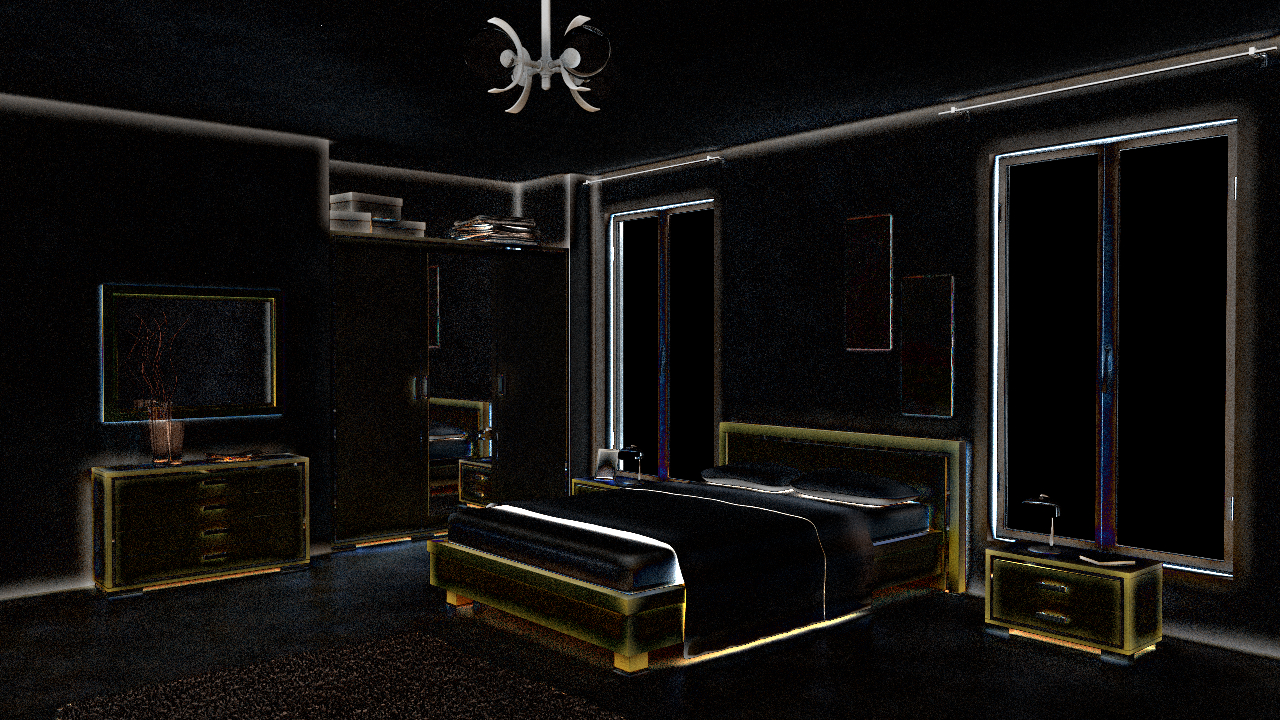
\includegraphics[width=1\textwidth]{evaluationResult/SPPM_PT/bedroom/rsebig.jpg}}
      \centerline{(b)}
    \end{minipage}    
    \caption{不同初始半径下的SPPM算法运算结果,其中(a)对应半径0.025,(b)对应半径0.15。两张图均以和路径追踪渲染结果之间的相对平方误差值来表示。}
    \label{fig:lab2compare}
\end{figure}

\section{VRay模拟材质效果测试}

关于VRay模拟材质,由于缺少精确的VRay材质公式、场景参数,且VRay渲染器对渲染结果做了许多后处理,
所以这里无法对双方的结果进行量化的比较。因此,本实验只放出双方的渲染结果,详见图\ref{fig:lab3compare}。

\begin{figure}                 %%%%%%%% 观测干扰的结果
    \begin{minipage}{0.40\textwidth}  %% {0.18\textwidth}
      \centerline{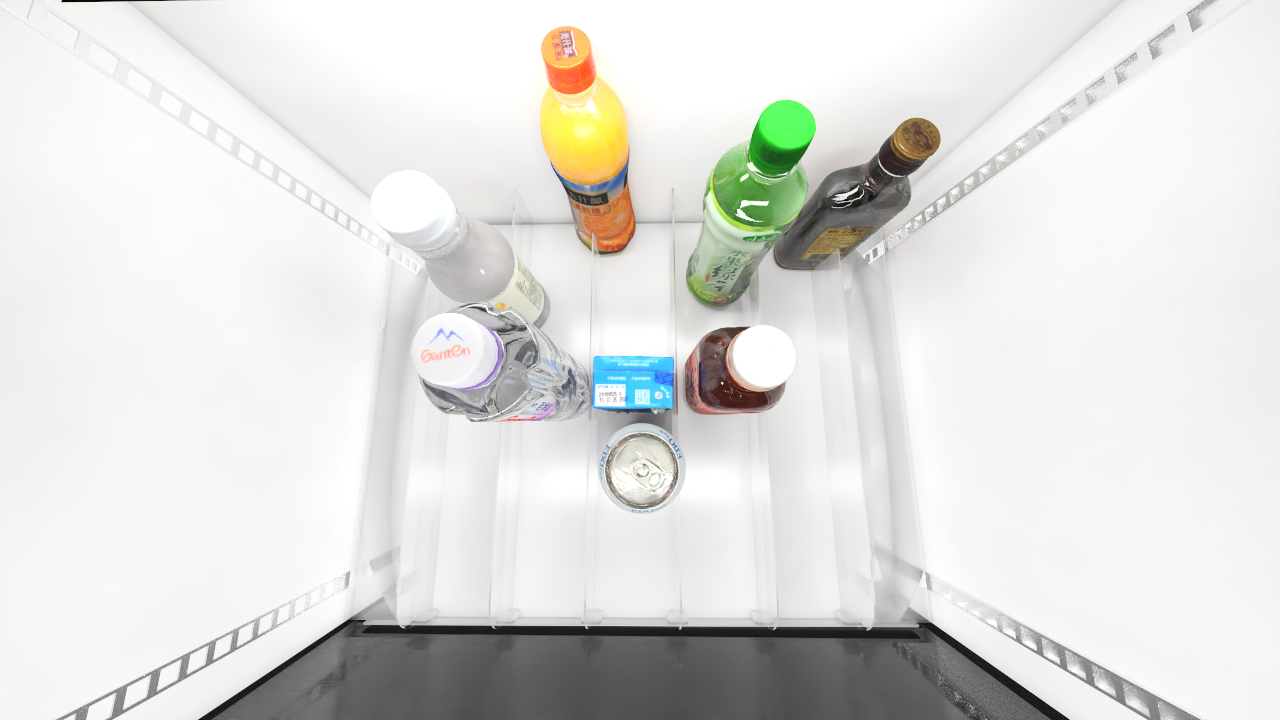
\includegraphics[width=1\textwidth]{evaluationResult/vray/1simulation.jpg}}
      \centerline{(a1)}
    \end{minipage}
    \hfill
    \begin{minipage}{0.40\textwidth}  %% {0.18\textwidth}
      \centerline{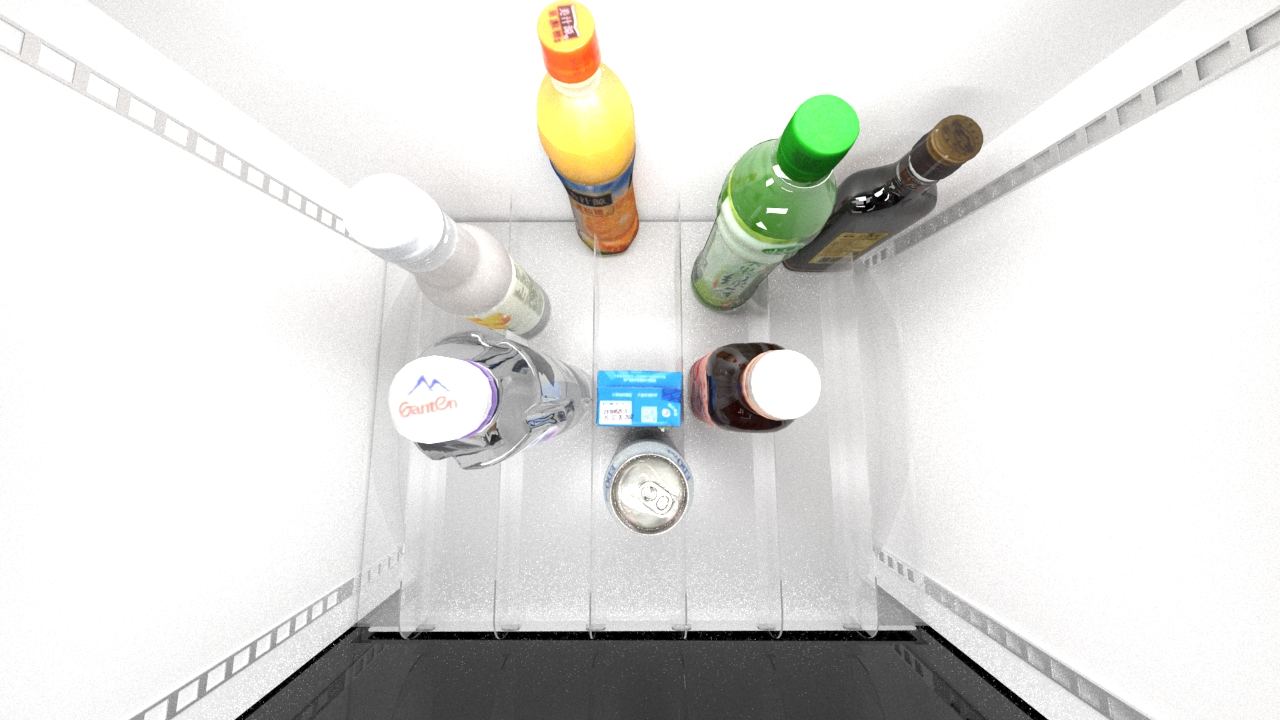
\includegraphics[width=1\textwidth]{evaluationResult/vray/1reference.jpg}}
      \centerline{(b1)}
    \end{minipage}
    \vfill
    \begin{minipage}{0.40\textwidth}  %% {0.18\textwidth}
        \centerline{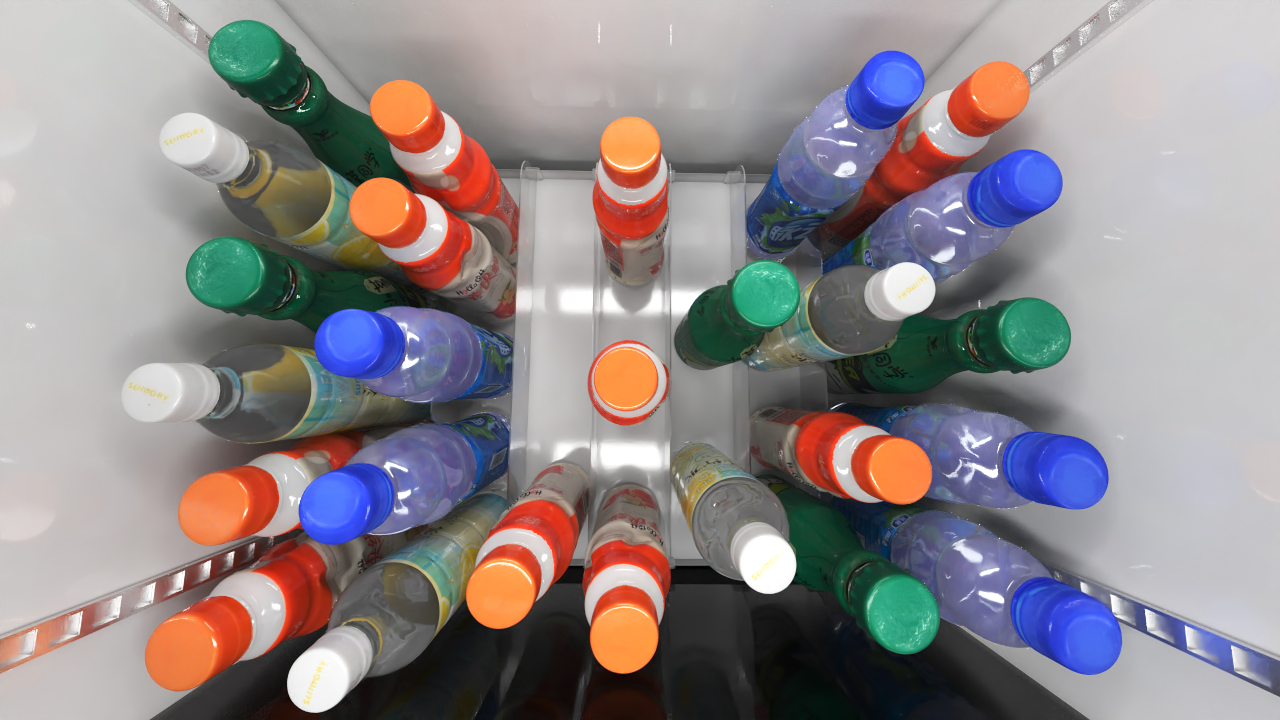
\includegraphics[width=1\textwidth]{evaluationResult/vray/2simulation.jpg}}
        \centerline{(a2)}
    \end{minipage}
    \hfill
    \begin{minipage}{0.40\textwidth}  %% {0.18\textwidth}
    \centerline{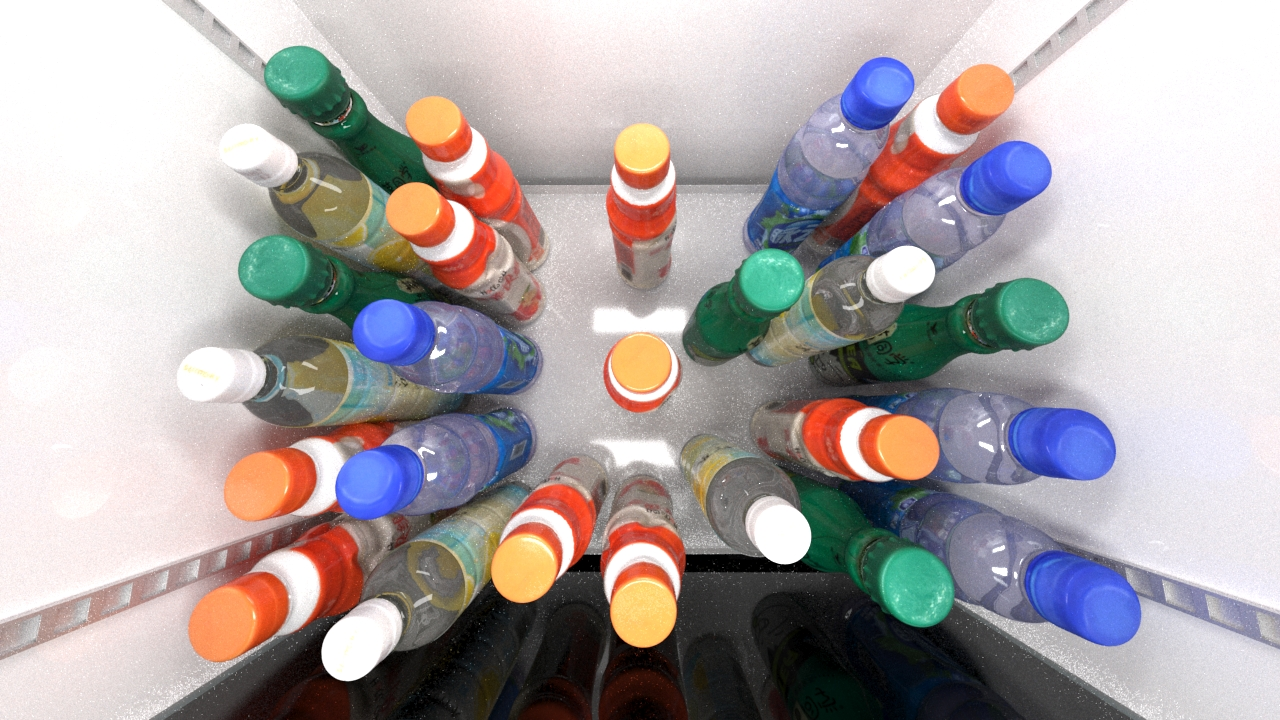
\includegraphics[width=1\textwidth]{evaluationResult/vray/2reference.jpg}}
    \centerline{(b2)}
    \end{minipage}
    \vfill
    \begin{minipage}{0.40\textwidth}  %% {0.18\textwidth}
    \centerline{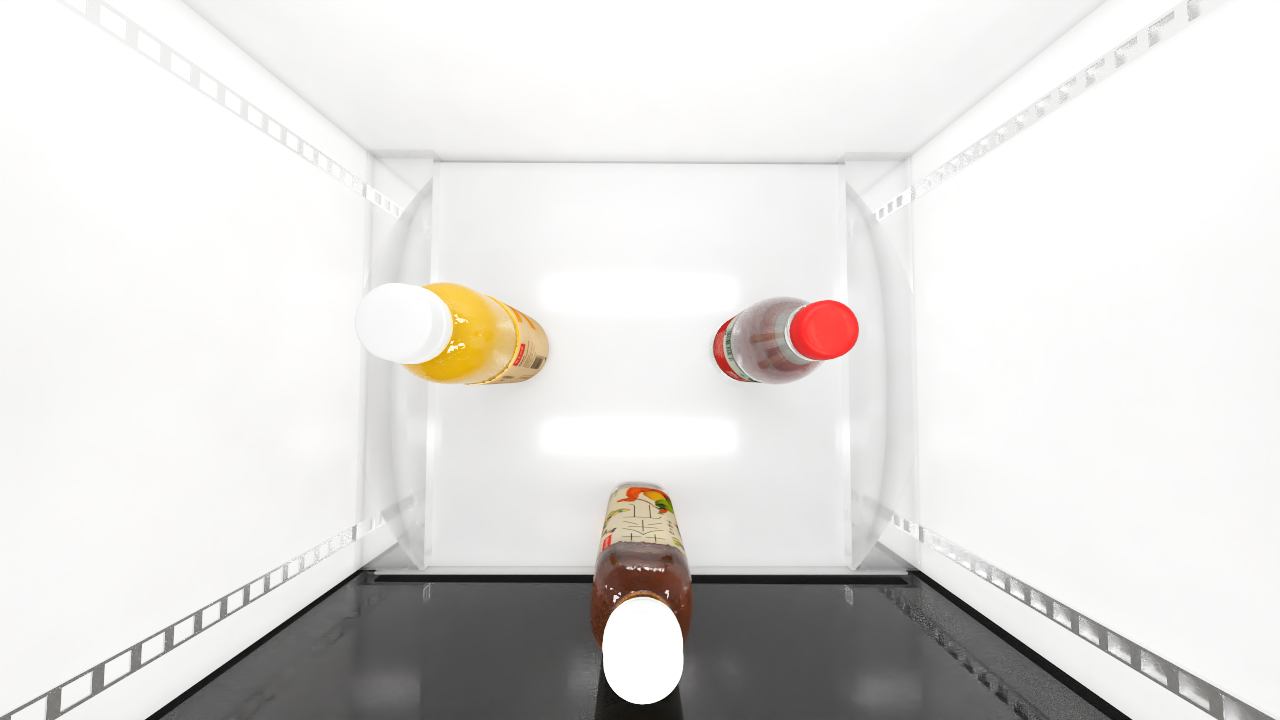
\includegraphics[width=1\textwidth]{evaluationResult/vray/3simulation.jpg}}
    \centerline{(a3)}
    \end{minipage}
    \hfill
    \begin{minipage}{0.40\textwidth}  %% {0.18\textwidth}
    \centerline{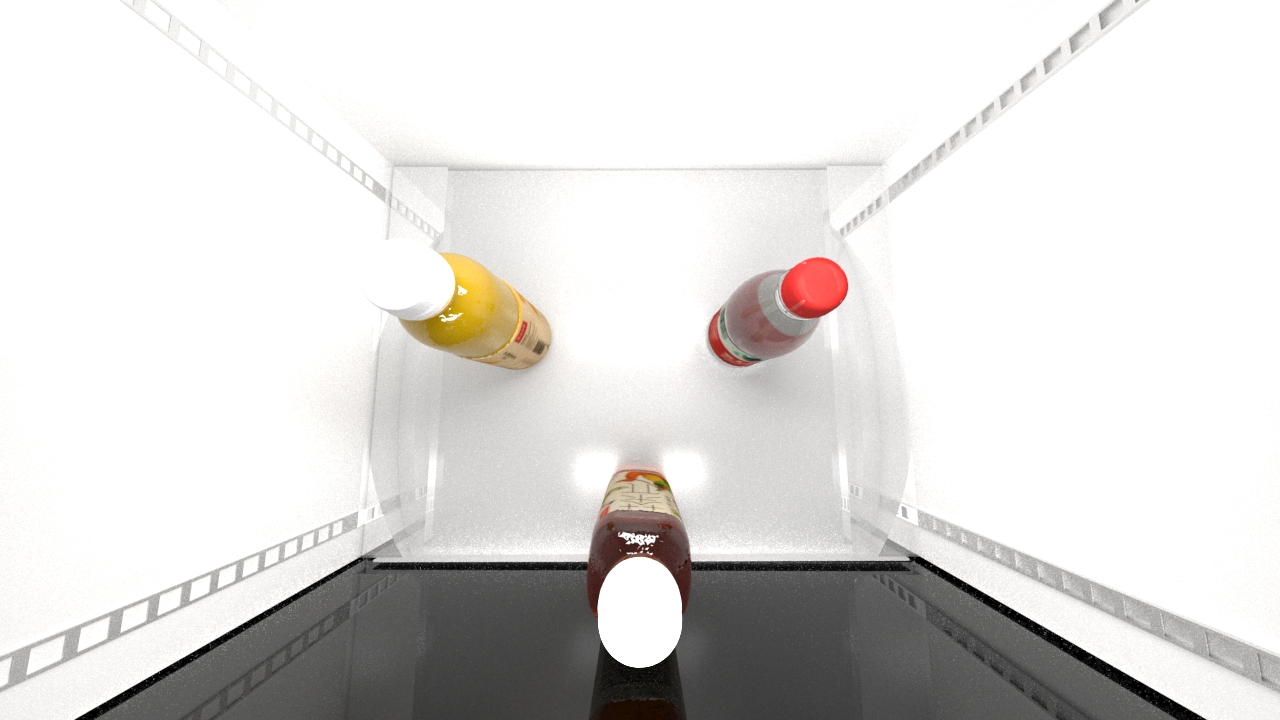
\includegraphics[width=1\textwidth]{evaluationResult/vray/3reference.jpg}}
    \centerline{(b3)}
    \end{minipage}    
    \vfill
    \caption{VRay模拟材质和实际材质的渲染结果。其中,左侧三张图(a1-a3)为模拟材质渲染结果,
    右侧三张图(b1-b3)为3ds max软件下的VRay渲染结果。}
    \label{fig:lab3compare}
\end{figure}

需要说明的是,有些结果图上的差异其实是由于双方渲染器中光源、摄像机等属性的实现方式不同而导致的,
与材质本身无关。
总体来看,VRay模拟材质的渲染效果已经和VRay原材质比较接近,
但在一些细节上(如半透明,一些材质的高光等)还存在部分偏差,需要进一步进行完善。

